\documentclass[a4paper,twoside,master.tex]{subfiles}
\begin{document}
\lecture{28}{Monday, March 30, 2020}{The Grand Canonical Ensemble}

Take a system at constant $ \{T,V,\mu\} $. Recall that
\begin{equation}
    \Omega(T,V, \mu) = U-TS- \mu N
\end{equation}
Note that this is equal to $ -PV $ if the system is extensive. Our microstate still contains $ N $ particles and six coordinates, so we still have a $ 6N $-dimensional phase space, but now $ N $ can vary. How do we deal with this? We can separate phase space into a collection of simple phase spaces at fixed $ N $ (\Cref{fig:lec_28_grand_canonical_phase_space}).

\begin{figure}[h]
    \centering
    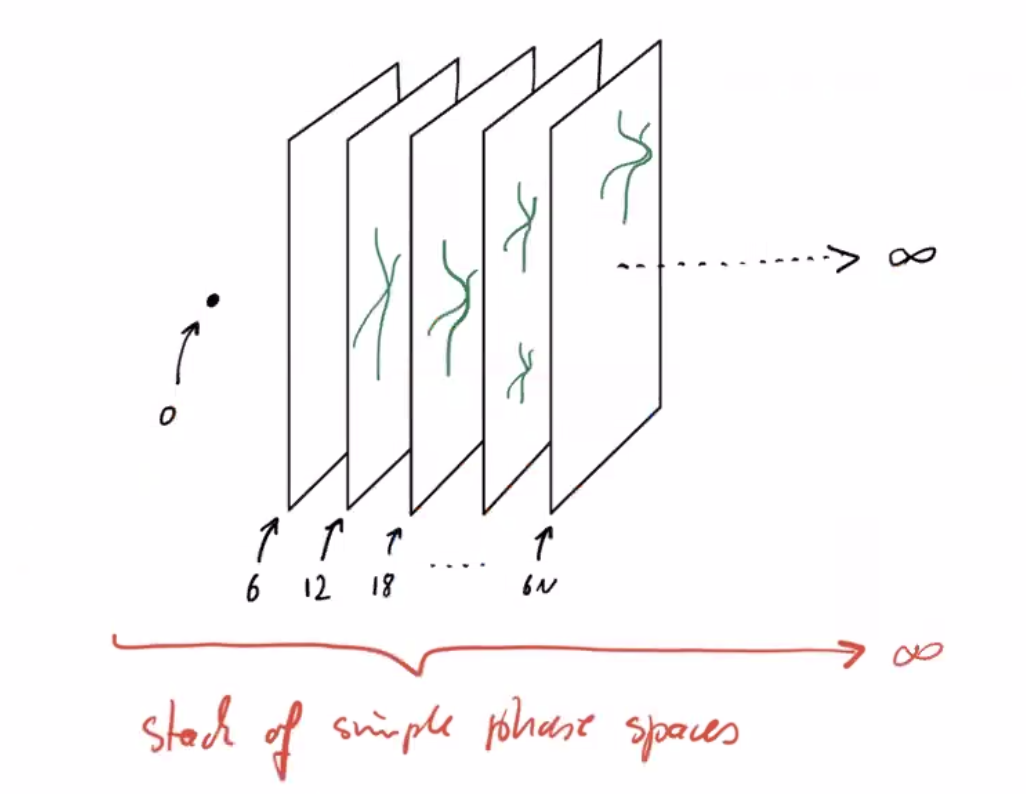
\includegraphics[width=\textwidth]{figures/lec_28_grand_canonical_phase_space.png}
    \caption{The Phase Space of the Grand Canonical Ensemble}
    \label{fig:lec_28_grand_canonical_phase_space}
\end{figure}

Our probability distribution can live anywhere on any of these planes, possibly in multiple places at the same time. To maintain our constant terms, we can imagine the system is in contact with a reservoir.
\begin{equation}
    P(E,N) = \frac{\Omega(E,V,N) \Omega_R(E_T - E, V_R, N_T - N)}{\Omega_T(E_T, V_T, N_T)}
\end{equation}
Here, let's say $ E << E_T $ and $ N << N_T $ and take the logarithm as we usually do:
\begin{align}
    \ln(P(E,N)) &= \ln(\Omega) + \ln(\Omega_R) - \ln(\Omega_T) \\
    &= \ln(\Omega) + \left[ \ln(\Omega_R(E_T, V_R, N_T)) - E \underbrace{\pdv{\ln(\Omega_R)}{E_T}}_{\beta} - N \underbrace{\pdv{\ln(\Omega_R)}{N_T}}_{- \beta \mu} + \ldots \right] - \ln(\Omega_T) \\
    &= \ln(\Omega) - \beta (E - \mu N) - \ln(\mathcal{Z})
\end{align}
so we can write
\begin{equation}
    P(E,N) = \frac{1}{\mathcal{Z}} \Omega(E,V,N) e^{- \beta (E - \mu N)}
\end{equation}
where
\begin{align}
    \mathcal{Z}(T,V, \mu) &= \sum_{N=0}^{\infty} \int \dd{E} \Omega(E,V,N) e^{- \beta (E - \mu N)} \\
    &= \sum_{N=0}^{\infty} Z(T,V,N) e^{\beta \mu N}
\end{align}
\begin{equation}
    \ln(\mathcal{Z}) = \underbrace{\frac{S}{k_B} - \beta (E - \mu N)}_{\sim N} - \underbrace{\ln(P(E,N))}_{\ln(N)}
\end{equation}
We will neglect the part that scales like $ \ln(N) $, so
\begin{equation}
    - k_B T \ln(\mathcal{Z}(T,V,NN)) = E - TS - \mu N = \Omega(T,V, \mu)
\end{equation}
where $ \Omega(T,V, \mu) $ is the grand potential (from back when we did transforms into things like enthalpy and the Gibbs free energy).

\begin{ex}
    Let's do an example with the ideal gas. Recall that we previously found
    \begin{equation}
        Z = \left( \frac{V}{\lambda^3_{\text{th}}} \right)^N \frac{1}{N!}
    \end{equation}
    and
    \begin{align}
        \mathcal{Z} &= \sum_{N=0}^{\infty} Z_N e^{\beta \mu N} = \sum_{N=0}^{\infty} \frac{1}{N!} \left( \frac{V}{\lambda^3_{\text{th}}} \right)^N e^{\beta \mu N} \\
        &= \exp\left\{ \frac{V e^{\beta \mu}}{\lambda^3_{\text{th}}} \right\}
    \end{align}
    \begin{equation}
        - PV = \Omega(T,V, \mu) = - k_B T \ln(\exp\left\{ \frac{V e^{\beta \mu}}{\lambda^3_{\text{th}}} \right\}) = - k_B T \frac{V}{\lambda^3_{\text{th}}} e^{\beta \mu}
    \end{equation}
    so
    \begin{equation}
        P_{\text{IG}}(T, \mu) = k_B T \frac{e^{\beta \mu}}{\lambda^3_{\text{th}}}
    \end{equation}
    or
    \begin{equation}
        \mu(T,P) = k_B T \ln\left( \frac{P \lambda^3_{\text{th}}}{k_B T} \right)
    \end{equation}
\end{ex}

\section{Quantum Statistical Physics}
\label{sec:quantum_statistical_physics}

Instead of looking at chapter 22, we will instead make some remarks on quantum mechanics within the context of statistical physics. We would like to first compare classical and quantum mechanics. For simplicity, let's only look at one Cartesian degree of freedom in a non-relativistic system with no spin.

\begin{tabular}{@{}lcc@{}}
    Concept & CM & QM \\
    \toprule
    Arena & Phase Space $ \Gamma $ ($ \cong \R^2 $) & Hilbert space $ \mathcal{H} $ ($ \cong L^2(\R) $) \\
    \midrule
    Canonical Variables & Real coordinates on $ \Gamma $, $ p $ and $ q $ & Self-adjoint operators on $ \mathcal{H} $, $ P $ and $ Q $ \\
    \midrule
    Elements of Liouville Space (Algebra) & Complex functions of $ \Gamma $ $ a(p,q) $ & Operators on Hilbert space $ A(P,Q) $ \\
    \bottomrule
\end{tabular}

\end{document}
